\documentclass[pdftex,12pt,a4paper]{article}

\usepackage{graphicx}  
\usepackage[margin=2.5cm]{geometry}
\usepackage{breakcites}
\usepackage{indentfirst}
\usepackage{pgfgantt}
\usepackage{pdflscape}
\usepackage{float}
\usepackage{epsfig}
\usepackage{epstopdf}
\usepackage[cmex10]{amsmath}
\usepackage{stfloats}
\usepackage{multirow}

\renewcommand{\refname}{REFERENCES}
\linespread{1.3}

\usepackage{mathtools}
%\newcommand{\HRule}{\rule{\linewidth}{0.5mm}}
\thispagestyle{empty}
\begin{document}
\begin{titlepage}
\begin{center}
\textbf{}\\
\textbf{\Large{ISTANBUL TECHNICAL UNIVERSITY}}\\
\vspace{0.5cm}
\textbf{\Large{COMPUTER ENGINEERING DEPARTMENT}}\\
\vspace{2cm}
\textbf{\Large{BLG 242E\\ DIGITAL CIRCUITS LABORATORY\\ EXPERIMENT REPORT}}\\
\vspace{2.8cm}
\begin{table}[ht]
\centering
\Large{
\begin{tabular}{lcl}
\textbf{EXPERIMENT NO}  & : & 4 \\
\textbf{EXPERIMENT DATE}  & : & 08.03.2019 \\
\textbf{LAB SESSION}  & : & FRIDAY - 14.00 \\
\textbf{GROUP NO}  & : & G13 \\
\end{tabular}}
\end{table}
\vspace{1cm}
\textbf{\Large{GROUP MEMBERS:}}\\
\begin{table}[ht]
\centering
\Large{
\begin{tabular}{rcl}{
150180704  & : & C\.{I}HAT AKK\.{I}RAZ \\
150180707  & : & FAT\.{I}H ALTINPINAR \\
150180734  & : & S\.{I}NAN \c{S}AR \\
}
\end{tabular}}
\end{table}
\vspace{2.8cm}
\textbf{\Large{SPRING 2019}}

\end{center}

\end{titlepage}

\newpage

\thispagestyle{empty}
\centering{\LARGE{ \textbf{ETHIC FORM}}}\\
\centering{\LARGE{\textbf{for}}}\\
\centering{\LARGE{\textbf{BLG242E Logic Circuits Laboratory}}}\\[0.2cm]
As a student of \\Istanbul Technical University Faculty of Computer and Informatics Engineering;
\begin{enumerate}
    \item I will not attempt to cheat in quizes and final exam,
    \item I will not use disallowed sources or tools (mobile phone, calculator etc.) during the exam,
    \item I will not write any information (formula, text, figure etc.) on the table, sheets or books that are allowed to be used during the exam,
    \item I will give reference when using printed or online published sources,
    \item I will not use the results in a source as they are, or by changing a part of them without giving a reference,
    \item I will not show unused sources as used, 
    \item I will not present someone else’s idea as my own idea, 
    \item I will not make someone do my homework, project or thesis for money or anything else,
    \item I will not take an exam or enter a lecture on behalf of others,
    \item I will not make excuses for not attending in exams or lessons by taking reports from someone I know (medical doctor parents or relatives),
    \item I will refrain from deliberately harming the public materials at our university,  
    \item I will comply with the safety rules in laboratory work,
    \item I will behave in accordance with the rules of respect for the lecturers and teaching assistants
\end{enumerate}
\vspace{-1em}
\centering{\LARGE{signed by}}\\
\vspace{-1em}
\begin{table}[ht]
\centering
\begin{tabular}{rcl}
150180704  & : & C\.{I}HAT AKK\.{I}RAZ \\
150180707  & : & FAT\.{I}H ALTINPINAR \\
150180734  & : & S\.{I}NAN \c{S}AR \\
\end{tabular}
\end{table}
\vspace{-1em}
 \begin{table}[ht]
 \begin{tabular}{lr}
%\textbf{Date:\hspace*{1.0cm}/\hspace*{1.0cm}/} &\qquad \qquad\qquad\qquad \qquad\qquad\qquad \qquad\qquad\qquad \qquad\qquad \textbf{SIGNED}\\
\end{tabular}
\end{table} % adds the ethic sign
\addcontentsline{toc}{section}{\numberline {}ETHICS}
\newpage

\thispagestyle{empty}
\addtocontents{toc}{\contentsline {section}{\numberline {}FRONT COVER}{}}
\addtocontents{toc}{\contentsline {section}{\numberline {}CONTENTS}{}}
\setcounter{tocdepth}{4}
\tableofcontents
\clearpage

\setcounter{page}{1}

\section{INTRODUCTION}
\begin{flushleft}
\paragraph{}
In this experiment, logic circuits are implemented to make arithmetic operations on signed and unsigned binary numbers. An Arithmetic Logic Unit(ALU) is used and some operations are made.
\end{flushleft}

\section{REQUIREMENTS}
\begin{flushleft}
\underline{Tools Used}\cite{booklet}
\end{flushleft}
\begin{itemize}
    \item C.A.D.E.T
    \item 74000 series ICs
    \begin{itemize}
        \item 74xx08 - Quadruple 2-input Positive AND Gates
        \item 74xx32 - Quadruple 2-input Positive OR Gates   
        \item 74xx83 - 4-bit Binary Full Adder
        \item 74xx86 - Quadruple 2-input Positive Exclusive Or (XOR) Gates
        \item 74xx174 - Hex D-Type Flip-Flops
        \item 74xx181 - 4-Bit Arithmetic Logic Unit
    \end{itemize}
\end{itemize}

\begin{flushleft}

\subsection{PART 1}
    \paragraph{}
    In the first part of the experiment, the circuit is designed as shown given diagram below. Logic switches are used for inputs and LED's on the monitor are used to observe output values.
    
      \begin{figure}[h]
    	\centering
    	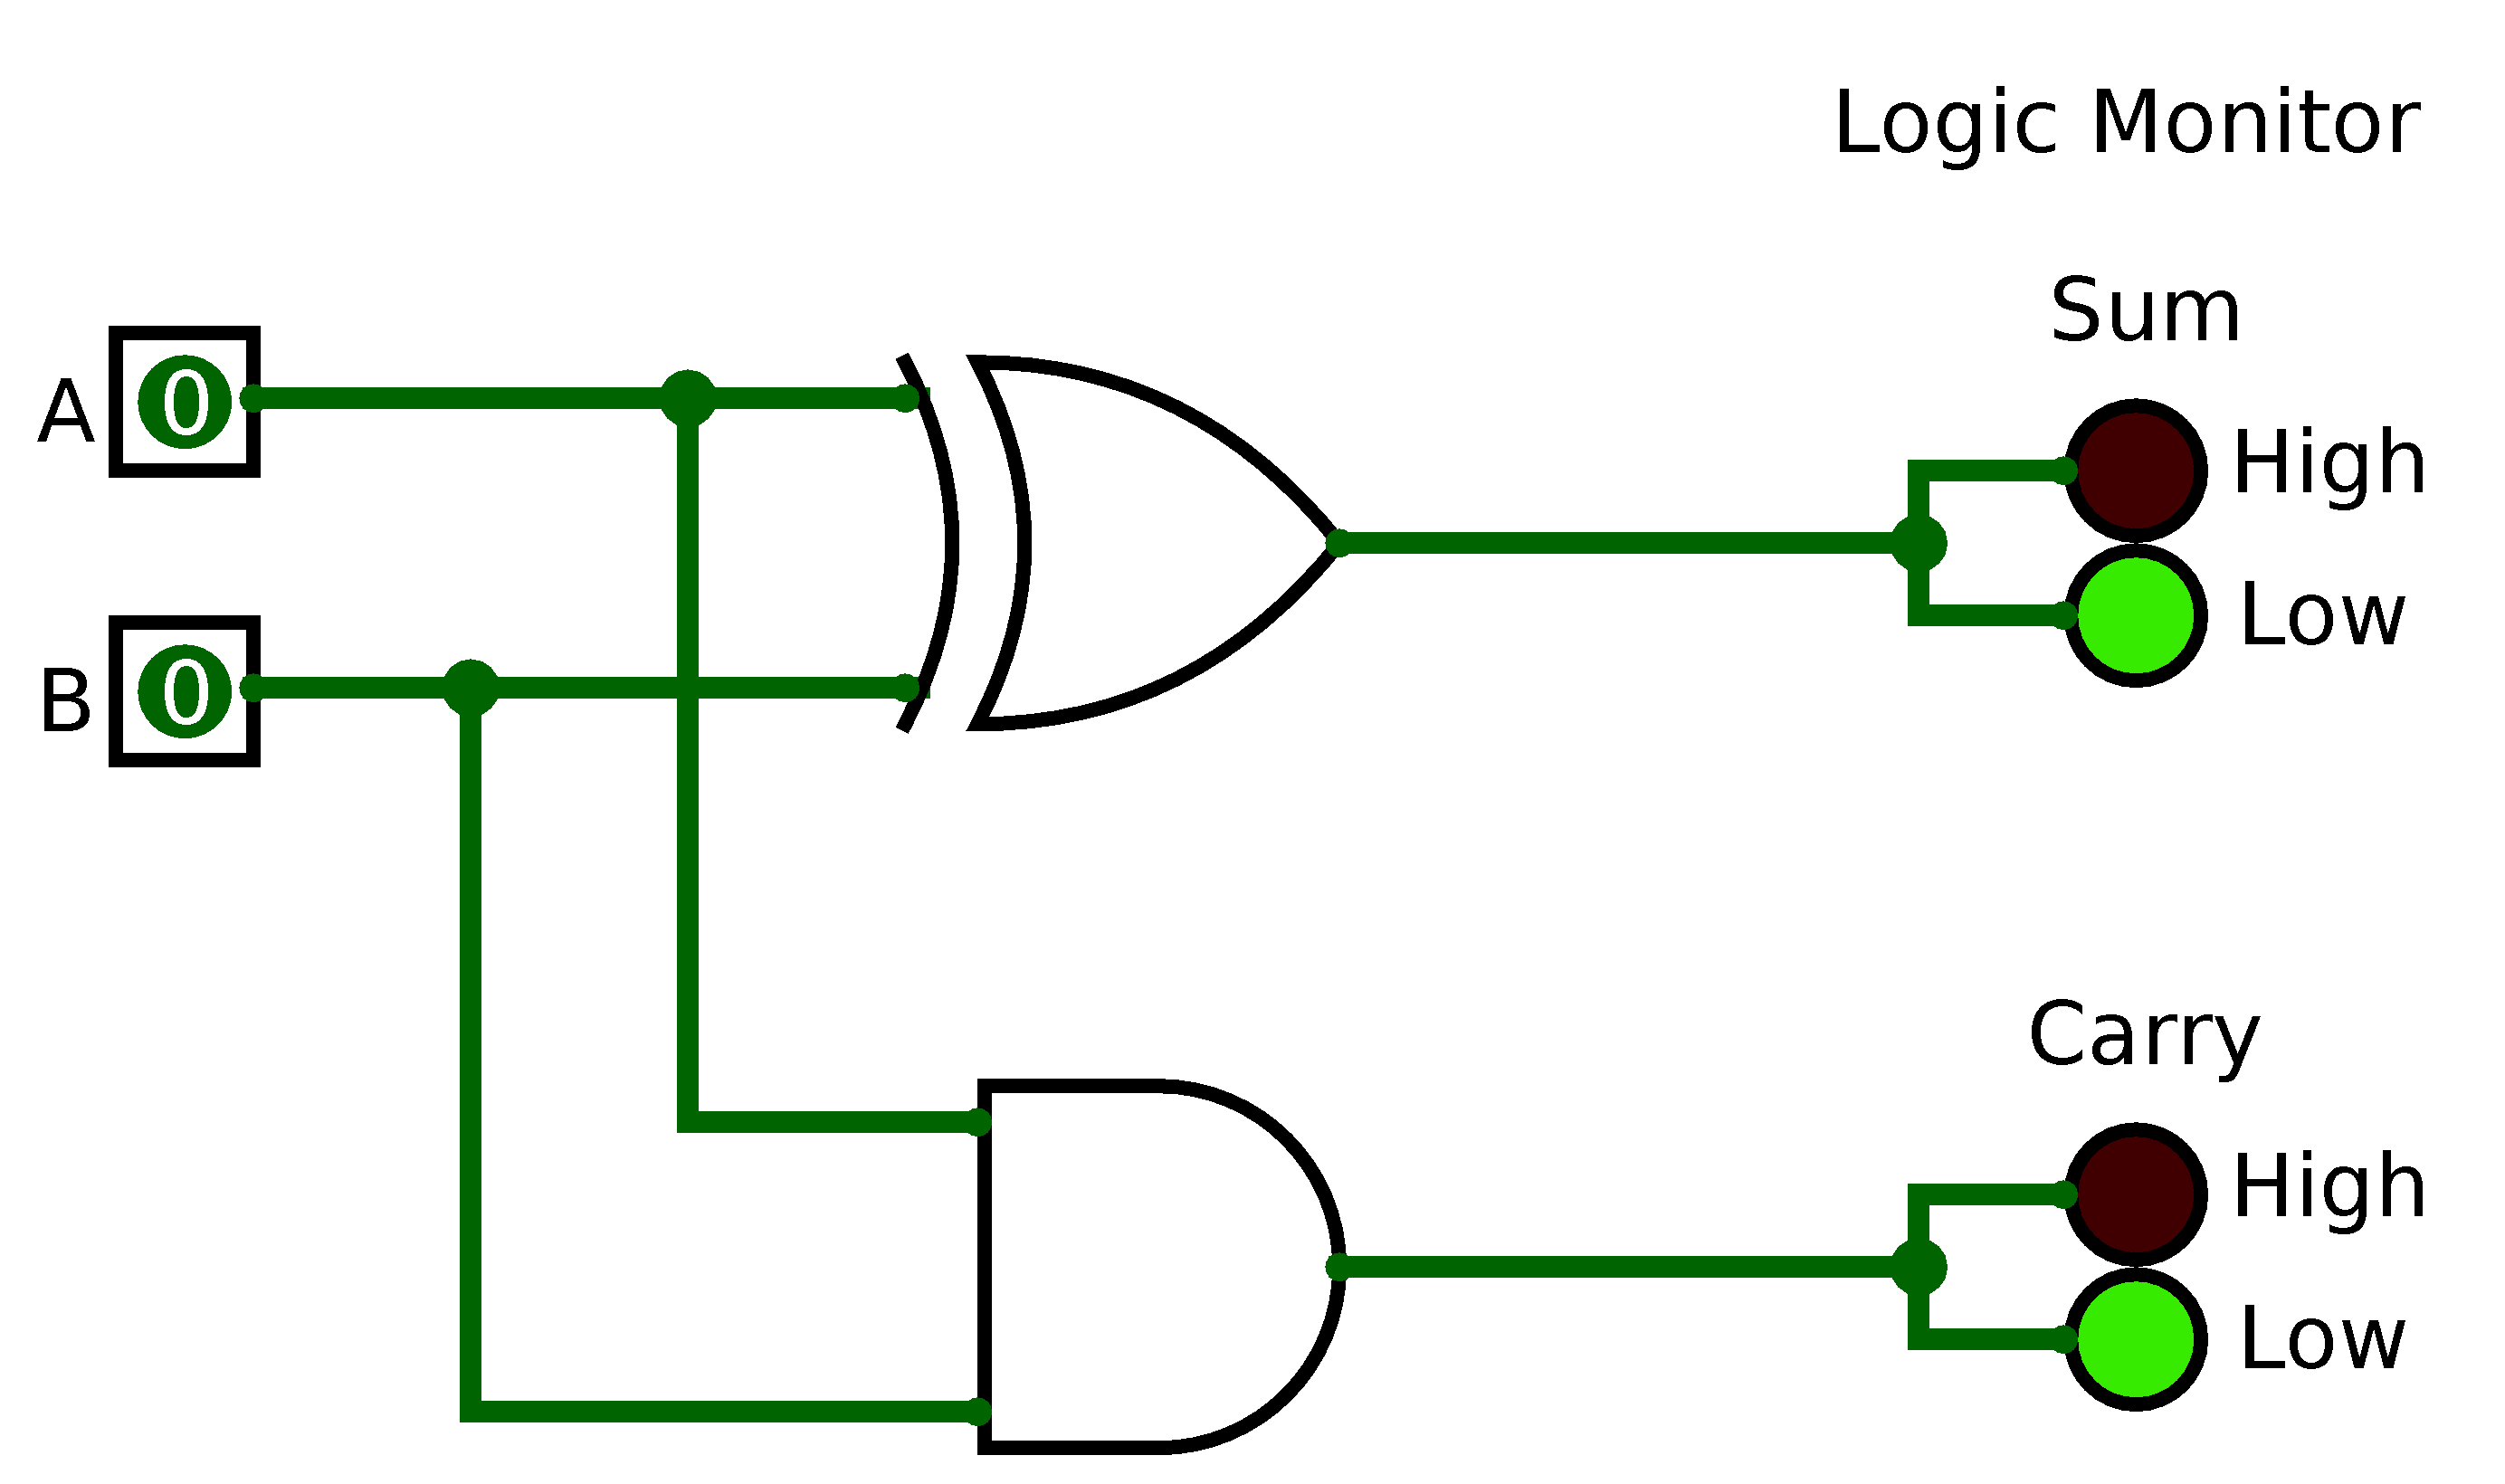
\includegraphics[width=0.5\textwidth]{part1.png}	
    	\caption{Half adder}
    	\label{fig:half_adder}
    \end{figure}
    \newpage
    \paragraph{}
    The output values of the circuit are validated with the truth table below.
    
    \begin{table}[!h]
    
\begin{center}
    \begin{tabular}{|c|c|c|c|}
    \hline
    
        \hline
         A & B & SUM & CARRY \\
         \hline
         0 & 0 & 0 & 0 \\
         \hline
         0 & 1 & 1 & 0 \\
         \hline
         1 & 0 & 1 & 0 \\
         \hline
         1 & 1 & 0 & 1 \\
         \hline
    \end{tabular}
    \caption{Truth table of half adder.}
    \label{table_half}
\end{center}
\end{table}
\subsection{PART 2}
    \paragraph{}
    In the next part of the experiment, some changes are made on the circuit which it's diagram was drawn in the previous part. One more input and additional gates are added to make the full adder circuit.
    
     \begin{figure}[h]
    	\centering
    	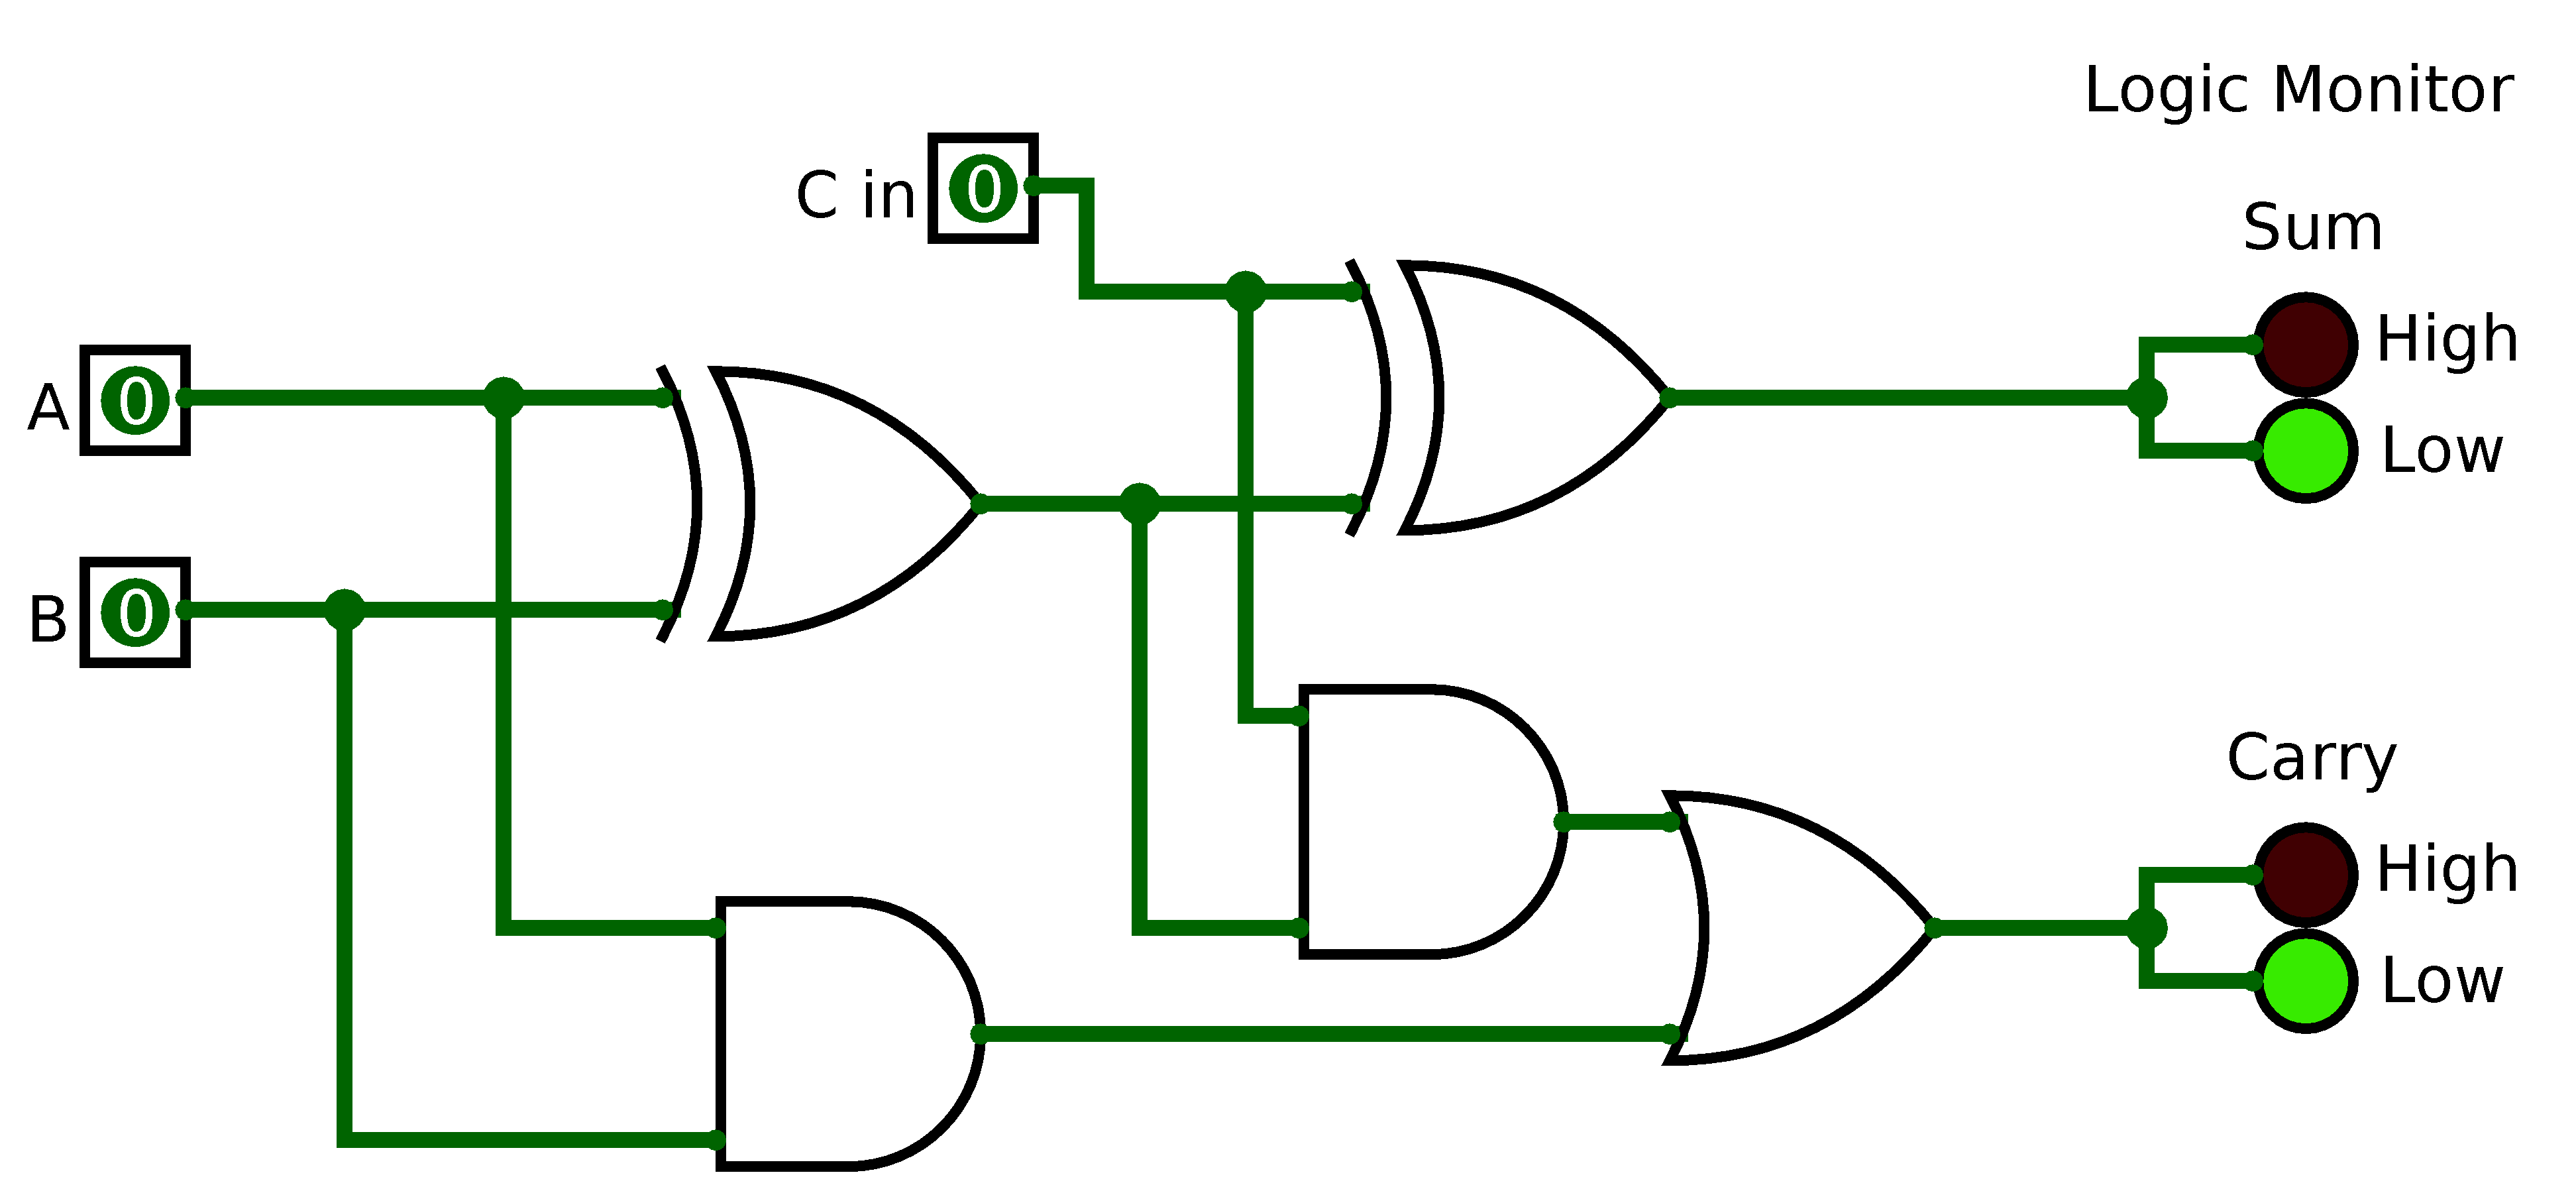
\includegraphics[width=0.5\textwidth]{part2.png}	
    	\caption{Full adder}
    	\label{fig:full_adder}
    \end{figure}
   
    \paragraph{}
    The output values of the circuit are validated with the truth table below.
    
\begin{table}[!h]
\begin{center}
    \begin{tabular}{|c|c|c|c|c|}
    \hline
    
        \hline
         A & B & $C_{in}$ & CARRY & SUM \\
         \hline
         0 & 0 & 0 & 0 & 0 \\
         \hline
         0 & 0 & 1 & 0 & 1 \\
         \hline
         0 & 1 & 0 & 0 & 1 \\
         \hline
         0 & 1 & 1 & 1 & 0 \\
         \hline
         1 & 0 & 0 & 0 & 1 \\
         \hline
         1 & 0 & 1 & 1 & 0 \\
         \hline
         1 & 1 & 0 & 1 & 0 \\
         \hline   
         1 & 1 & 1 & 1 & 1 \\
         \hline         
    \end{tabular}
    \caption{Truth table of full adder.}
    \label{table_full}
\end{center}
\end{table}    

\newpage

\subsection{PART 3}
\paragraph{}
In the next part of the experiment, the circuit is implemented using a 4-bit full adder(74xx83) as shown diagram below. The output values(Carry and Sum) are observed for some test cases given in the booklet. Addition and subtraction operations are made and output values are interpreted considering both signed and unsigned input values. 

 \begin{figure}[h]
    	\centering
    	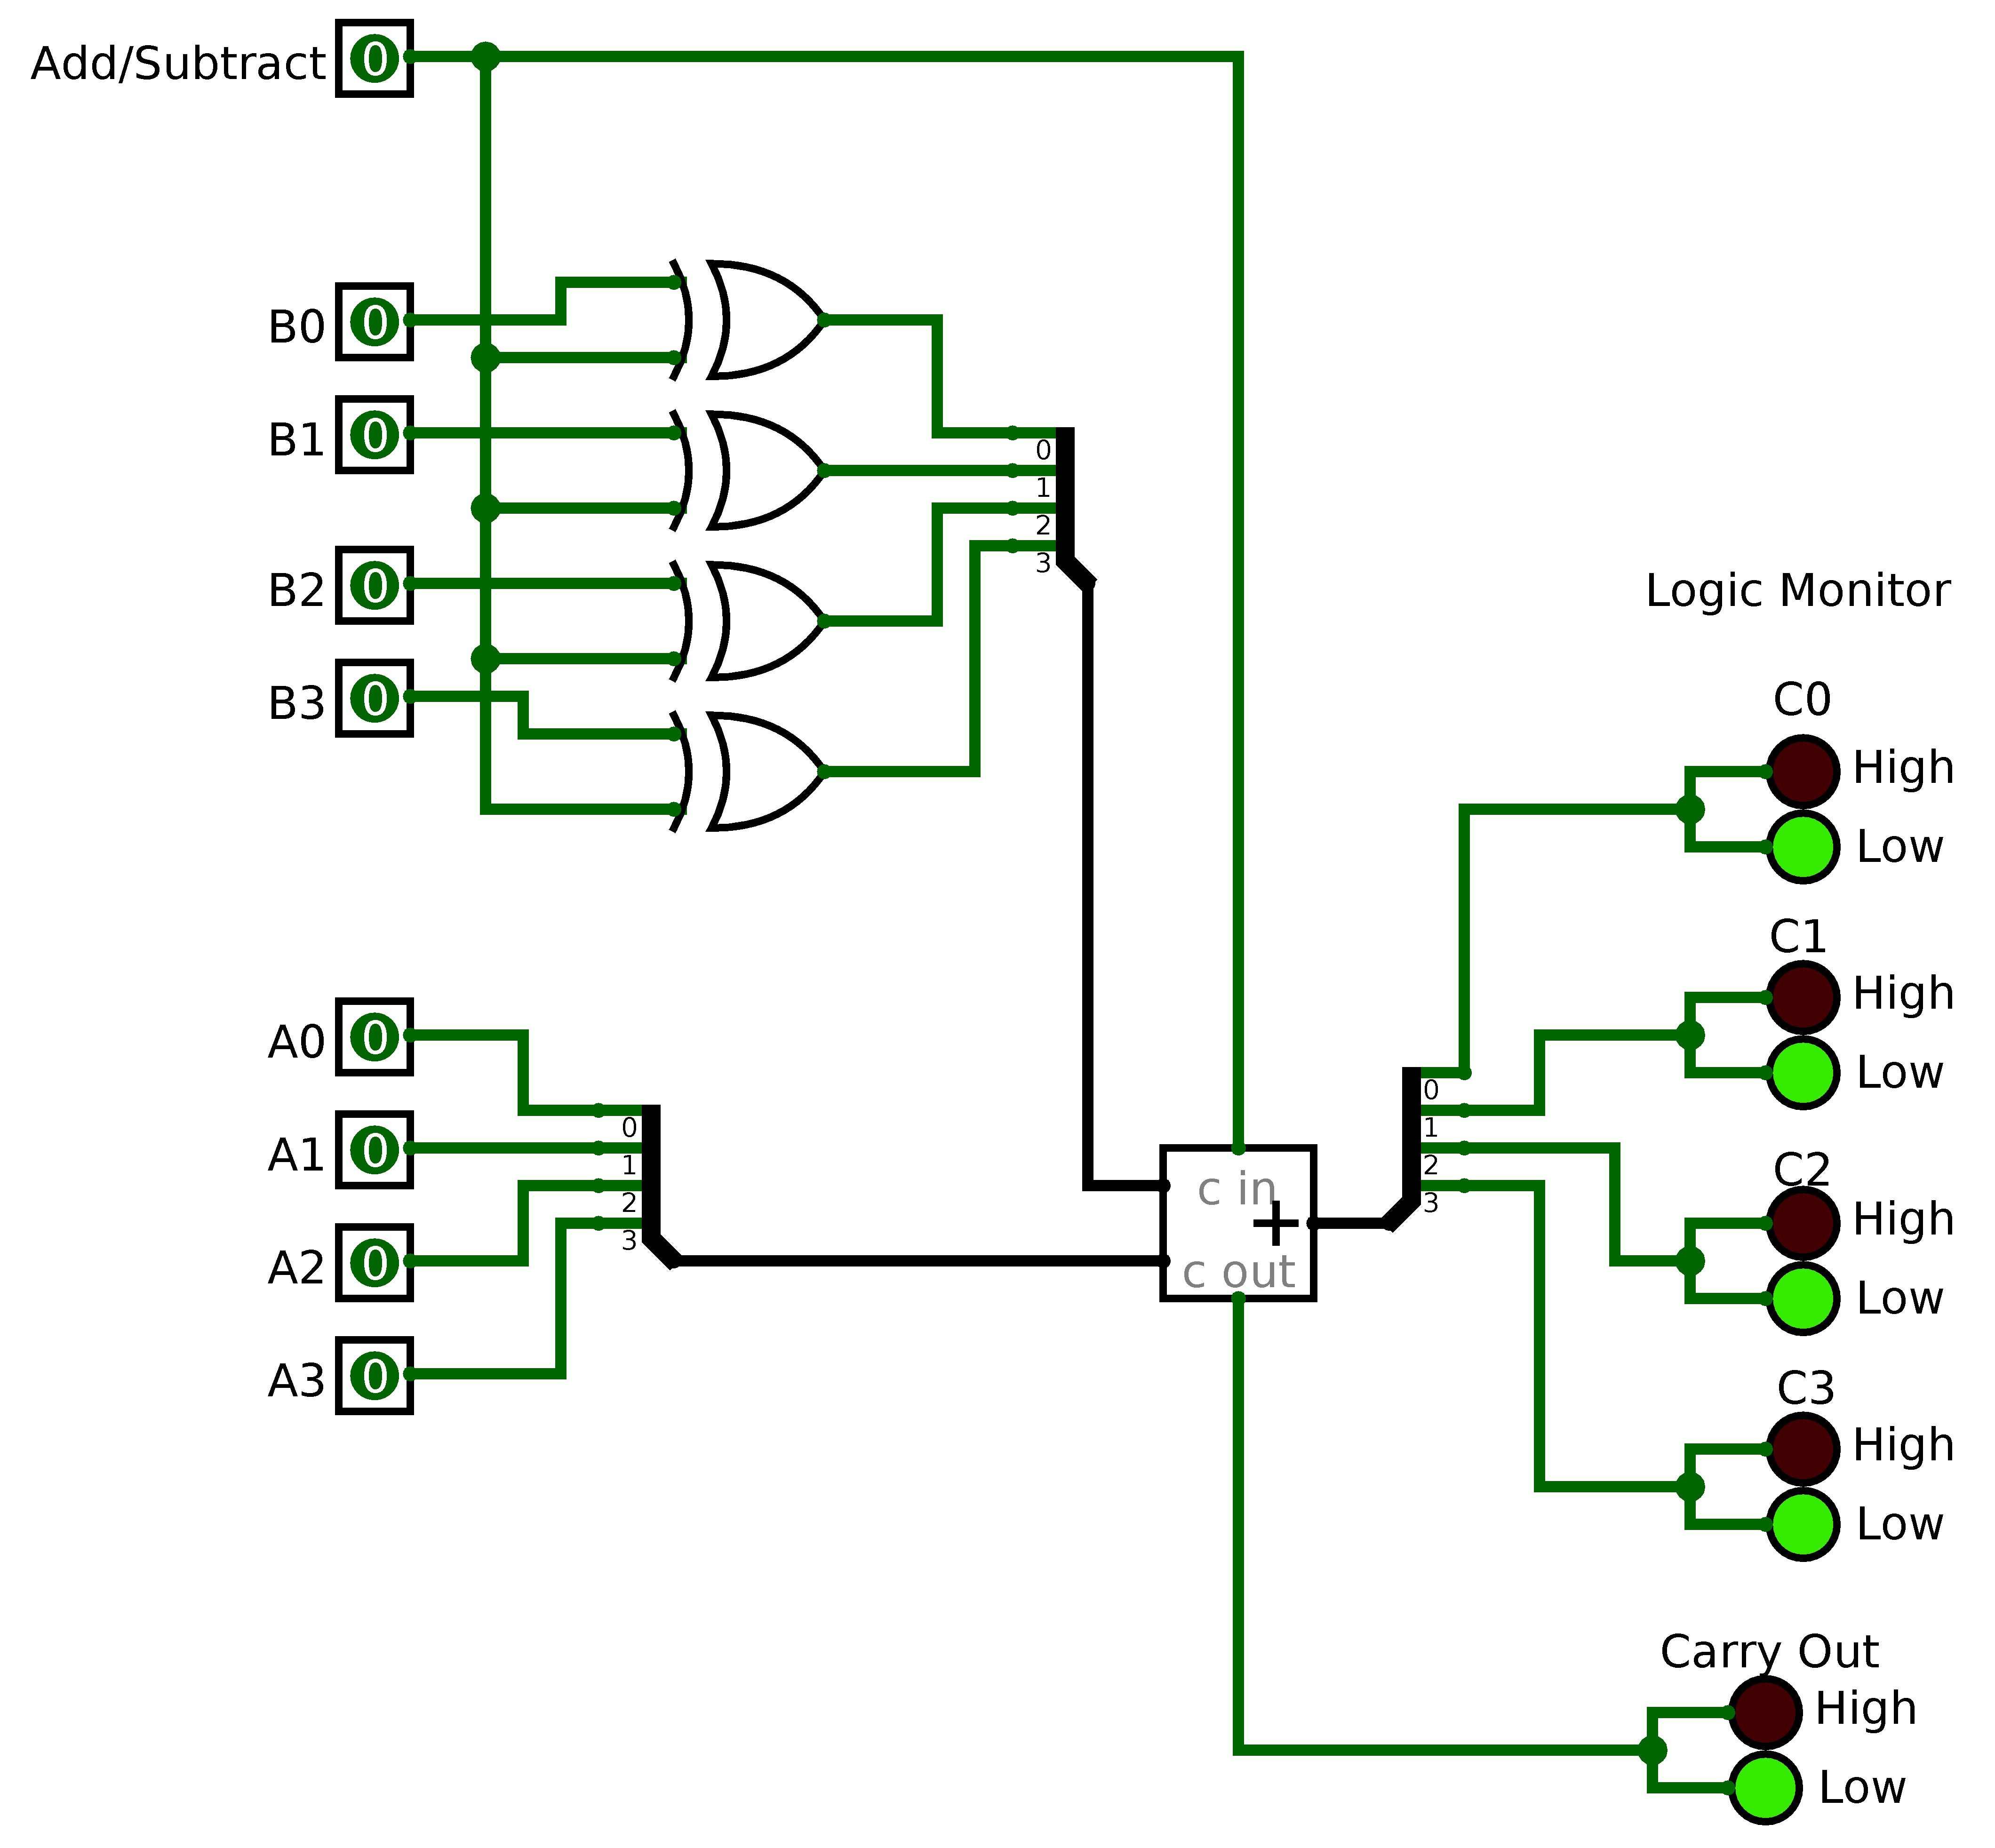
\includegraphics[width=0.5\textwidth]{part3.png}	
    	\caption{4 bit full adder}
    	\label{fig:4-bit_full_adder}
    \end{figure}


% TEST CASES
\begin{table}[h]
\begin{center}
    \begin{tabular}{|c|c|c|c|c|}
    \hline
         Test Case & 1 & 2 & 3 & 4  \\
         \hline
         A & 0101 & 1101 & 1111 & 0110 \\
         \hline
         B & 0111 & 1001 & 1111 & 1101 \\
         \hline
    \end{tabular}
    \caption{Test cases for arithmetic operations.}
    \label{truthtablep1}
\end{center}
\end{table}

\begin{table}[!h]
\begin{center}
    \begin{tabular}{|c|c|c|c|c|}
    \hline
         A & B & Carry & Result in Binary & Result in Decimal \\
         \hline
         0101 & 0111 & 0 & 1100 & 12 \\
         \hline
         1101 & 1001 & 1 & 0110 & 22  \\
         \hline
         1111 & 1111 & 1 & 1110 & 30 \\
         \hline
         0110 & 1101 & 1 & 0011 & 19 \\
         \hline
        \end{tabular}
    \caption{Results of the unsigned sum $A + B$.}
    \label{unsigned_sum}
\end{center}
\end{table}


\paragraph{}
In Table \ref{unsigned_sum}, output values that obtained addition operation are interpreted as unsigned input values. It is observed that for the first case there is no carry and result can be represented with 4 bit but for the other cases result cannot be represented with 4 bit and fifth bit(carry bit) is necessary.

\begin{table}[!h]
\begin{center}
    \begin{tabular}{|c|c|c|c|c|c|}
    \hline
         A & B & Overflow & Result sign & Result in Binary & Result in Decimal \\
         \hline
         0101 & 0111 & 1 & - & 1100 & -4 \\
         \hline
         1101 & 1001 & 1 & + & 0110 & 6 \\
         \hline
         1111 & 1111 & 0 & - & 1110 & -2 \\
         \hline
         0110 & 1101 & 0 & + & 0011 & 3 \\
         \hline
        \end{tabular}
    \caption{Results of the signed sum $A + B$.}
    \label{signed_sum}
\end{center}
\end{table}

\paragraph{}
In the Table \ref{signed_sum}, output values that obtained addition operation are interpreted as signed input values. It is observed that results are not valid for the four cases. Overflow occurs for the first and second cases because signs of the input values are same but signs of the output values are different. 
\begin{table}[!h]
\begin{center}
    \begin{tabular}{|c|c|c|c|c|}
    \hline
         A & B & Borrow & Result in Binary & Result in Decimal \\
         \hline
         0101 & 0111 & 1 & 1110 & 14 \\
         \hline
         1101 & 1001 & 0 & 0100 & 4 \\
         \hline
         1111 & 1111 & 0 & 0000 & 0 \\
         \hline
         0110 & 1101 & 1 & 1001 & 9 \\
         \hline
        \end{tabular}
    \caption{Results of the unsigned subtraction $A - B$}
    \label{unsigned_subtract}
\end{center}
\end{table}

\paragraph{}
In the Table \ref{unsigned_subtract}, output values that were obtained by subtraction operation are interpreted as unsigned input values. It is observed that result is  valid for the second and third cases and is not valid for the first and fourth cases by reason of presence of borrow. If there is a borrow this means second number is larger than the first one. The result which should be a negative number, cannot be represented with unsigned numbers.

\begin{table}[!h]
\begin{center}
    \begin{tabular}{|c|c|c|c|c|c|}
    \hline
         A & B & Overflow & Result sign & Result in Binary & Result in Decimal \\
         \hline
         0101 & 0111 & 0 & - & 1110 & -2 \\
         \hline
         1101 & 1001 & 0 & + & 0100 & 4 \\
         \hline
         1111 & 1111 & 0 & + & 0000 & 0 \\
         \hline
         0110 & 1101 & 1 & - & 1001 & -7 \\
         \hline
        \end{tabular}
    \caption{Results of the signed subtraction $A - B$}
    \label{signed_subtraction}
\end{center}
\end{table}

\paragraph{}
In the Table \ref{signed_subtraction}, output values that obtained subtraction operation are interpreted as signed input values. It is observed that result is valid for all cases except the fourth one. Fourth case is not valid since subtracting a negative number from a positive one should yield a positive number. As can be seen in the table result is negative, which means overflow. 


\subsection{PART 4}

\paragraph{}

In the final part of the experiment, the circuit shown below is implemented using a 4-Bit Arithmetic Logic Unit(74xx181) and a D type flip-flop(74xx174). Also hex inverters are used because of the fact that $F$ outputs of ALU are in negative logic. Input values are controlled by the logic switches and output values are observed on the logic monitor LED's on the C.A.D.E.T. Clock, M, and clear are controlled by the logic switches as well. Cn input of ALU is connected to ground(0V).



\end{flushleft}
\begin{figure}[h]
    	\centering
    	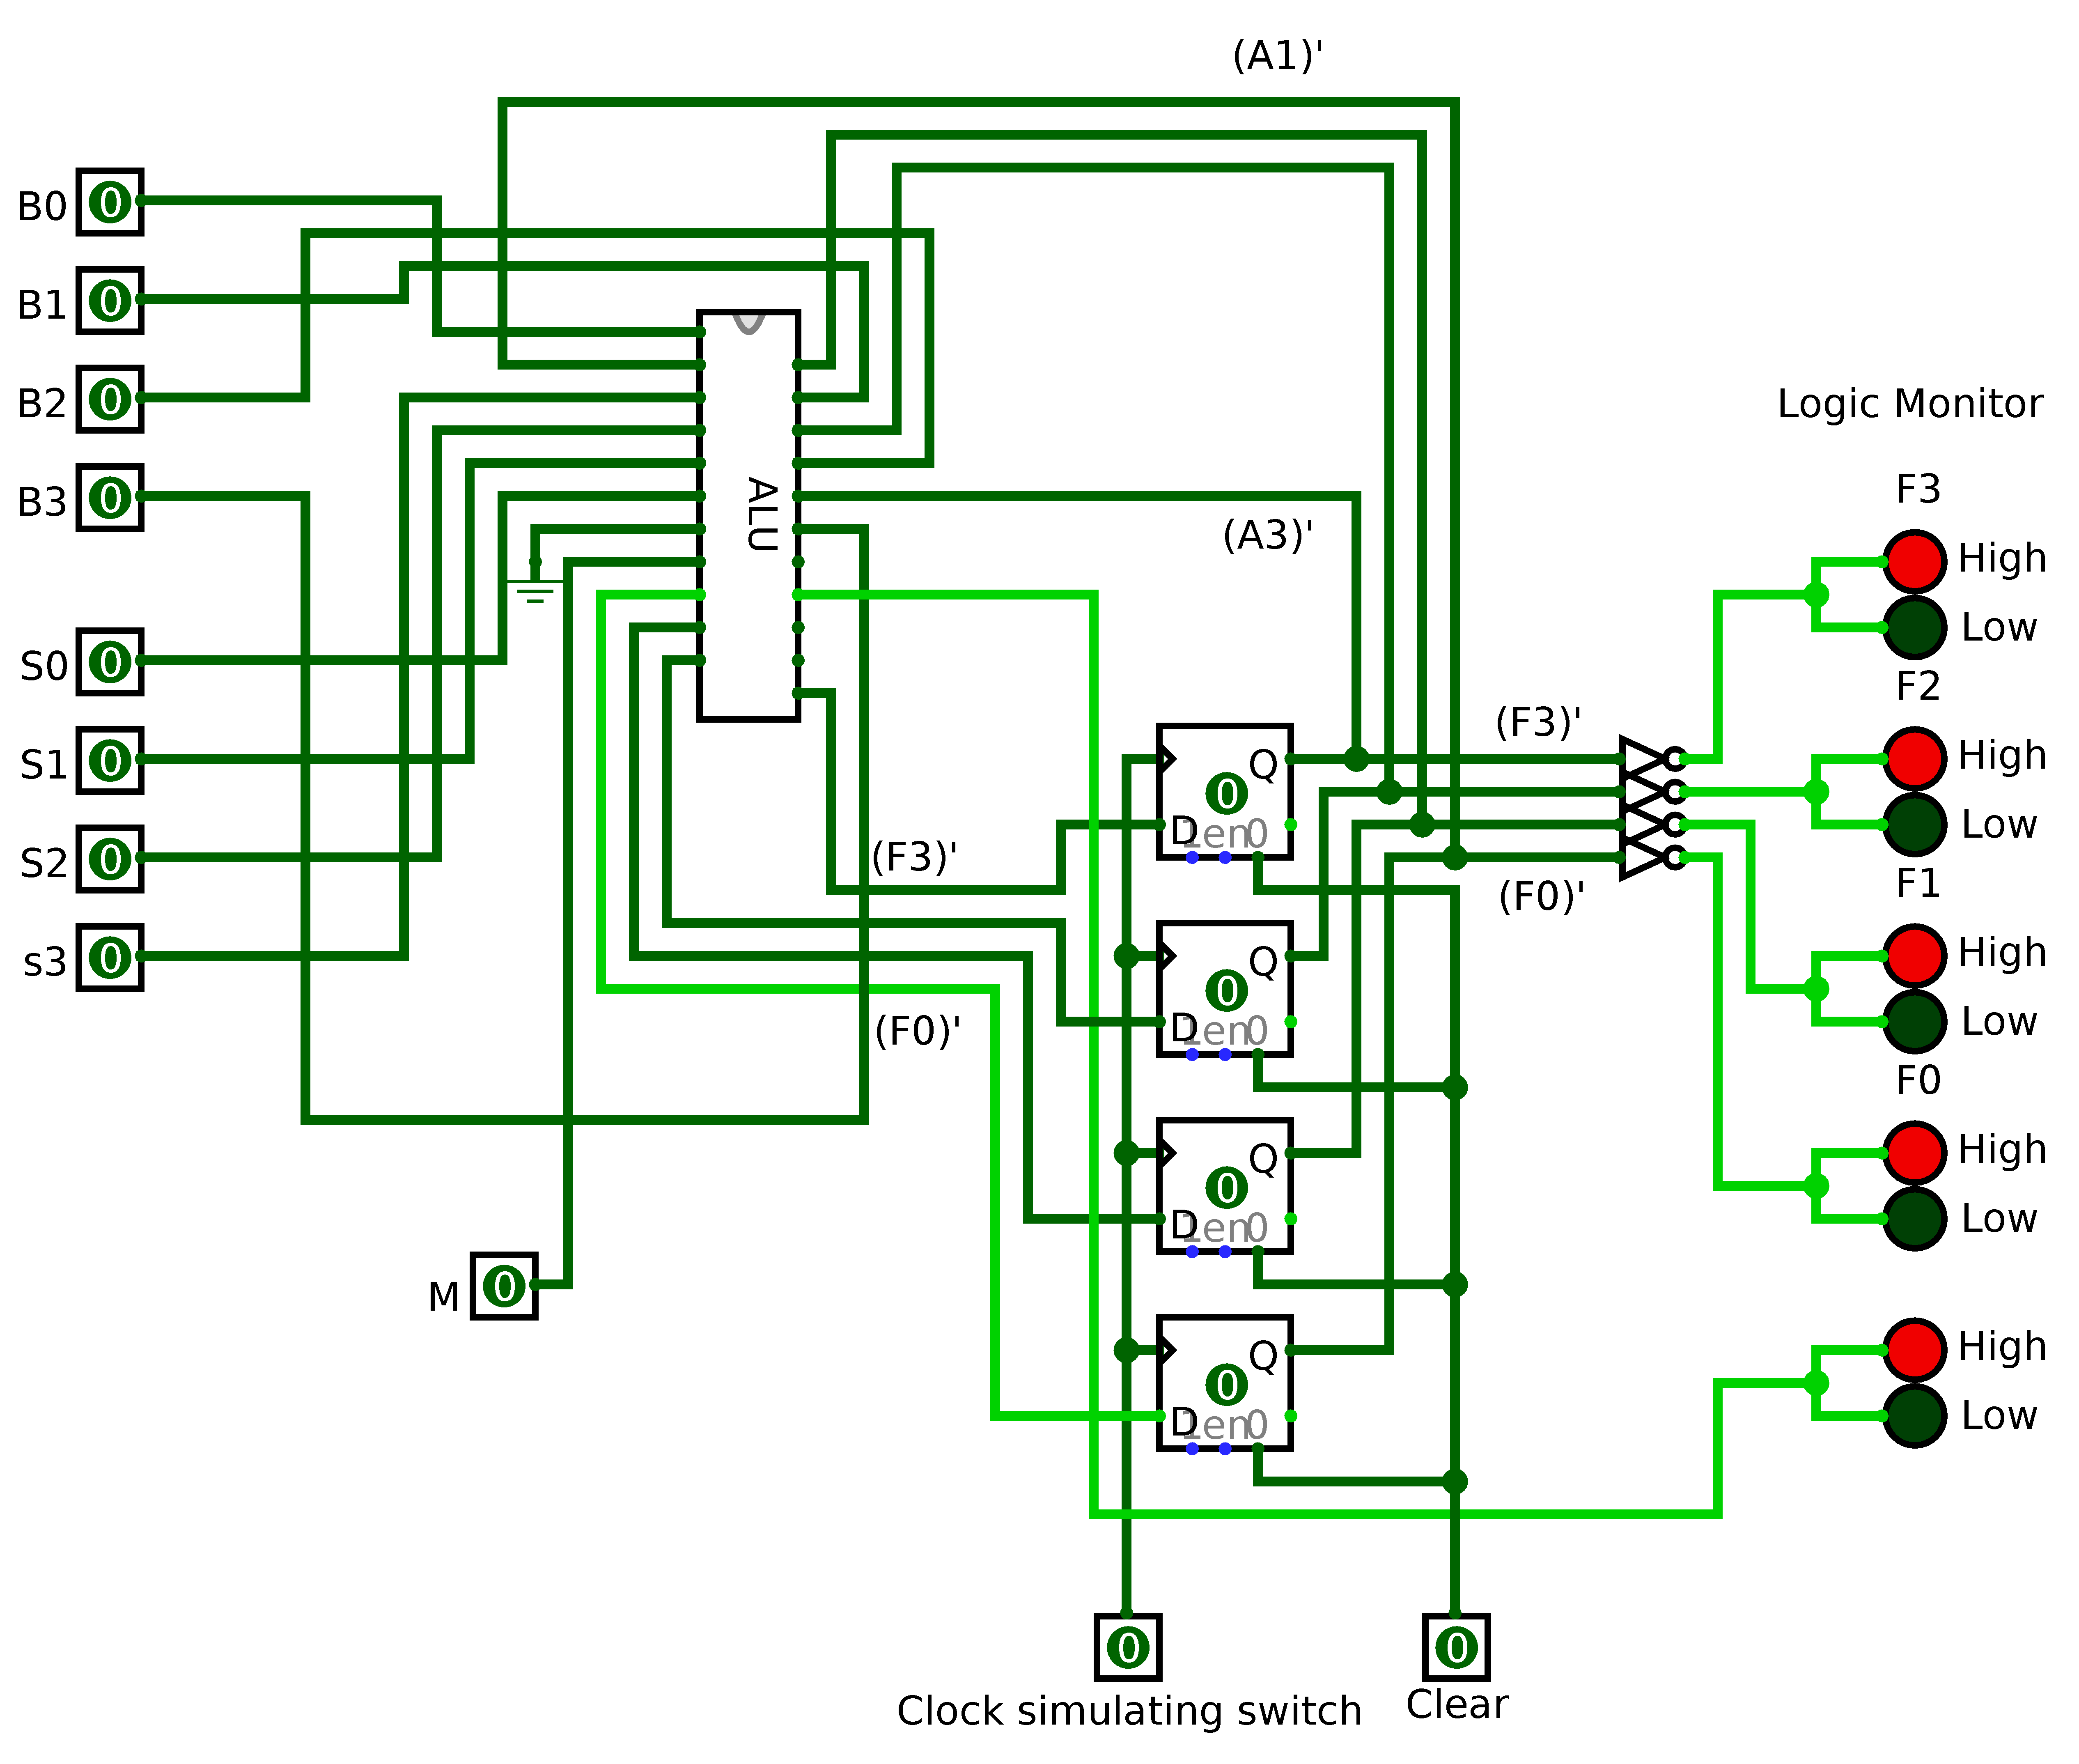
\includegraphics[width=1\textwidth]{part4.png}	
    	\caption{4 bit full adder}
    	\label{fig:4-bit_full_adder}
    \end{figure}

\newpage
\section{INTERPRETATION OF THE RESULTS}
%damn this is tough!
\begin{flushleft}

\paragraph{}
In the first three parts of this experiment results were consistent with our calculations and our circuits worked without any problems.(Detailed information about design process and theory for each part is presented in the sections above.) For the 4th part, we did not get the result we expected. We believe that, this was caused by a problem that occured while we incorporated the flip flop in our design. 
\end{flushleft}
\section{CONCLUSION}
\begin{flushleft}

\paragraph{}
Except for the fourth part of the experiment, no problems occured through the experiment. We were able to observe the results desired and go through parts 1,2 and 4 pretty quickly. In part 4, we designed a circuit and built it on the breadboard. We were able to set values to the ALU with no problems occuring but addition operation did not work the way it was supposed to. Therefore we dissembled the circuit and built it from the start once again, that would have solved the issue in the case where it was about the cables. But that didn't work, so we decided to change the design. We made adjustments to the outputs of the D-Flip Flop 2 but unfortunately we couldn't find the problem and weren't able to fully complete the part.
\end{flushleft}
\newpage
\addcontentsline{toc}{section}{\numberline {}REFERENCES}

\bibliographystyle{unsrt}
\bibliography{reference}

\end{document}

